\chapter{Introduction}

% Problem landscape
Engineering design is the disciplined process of transforming needs and requirements into realizable artifacts--such as structures, machines or systems--under various performance, safety, cost, manufacturability and regulatory constraints. Design choices determine whether a system can be built safely and economically, how efficiently it will operate over its lifetime, and how well it meets societal goals like sustainability and reliability. Over the past decades, engineers have increasingly adopted Computer-Aided Design and Engineering (CAD/CAE) tools that use computational models to sketch products and then predict how candidate designs will behave under real-world conditions before real fabrication. CAD/CAE technologies improve design accuracy and efficiency, reduce reliance on costly physical prototypes, and enable systematic exploration of alternatives, making modern high-performance design feasible at industrial scale.

Despite these advances, designing complex 3D objects from scratch remains a labor-intensive, time-consuming task. Modern design processes are inherently multidisciplinary, requiring simultaneous consideration of various demands and constraints, such as performance, manufacturability and usability. These complexities are further amplified by high-dimensional design spaces, where physics (e.g., fluid dynamics, structural mechanics) and geometries must be seamlessly integrated. As a result, traditional engineering design remains a multi-step, expert-intensive process. As illustrated in Figure~\ref{ch1:fig:traditional_framework}, a typical workflow begins with design identification, where business, manufacturing, and regulatory requirements are translated into design objectives and constraints. Next comes an iterative conceptual design phase, through architecting, synthesis and refinement, to define the basic configuration (overall layout, shape and composition). Finally, design optimization adds another loop of meshing, simulation, and shape editing to fine-tune geometry for physical performance. At each stage, extensive reliance on specialists across different disciplines and domain-specific tools makes the workflow costly, slow and hard to scale. When applied to industrial practice, such serial manual workflows involving experts across domains lead to high costs in training, communication and management. Human factors such as fatigue, inexperience and inconsistency can contribute to $20\%$ of total operational costs[4], often leading to time and budget overruns.

\begin{figure}[tbh]
    \begin{center}
        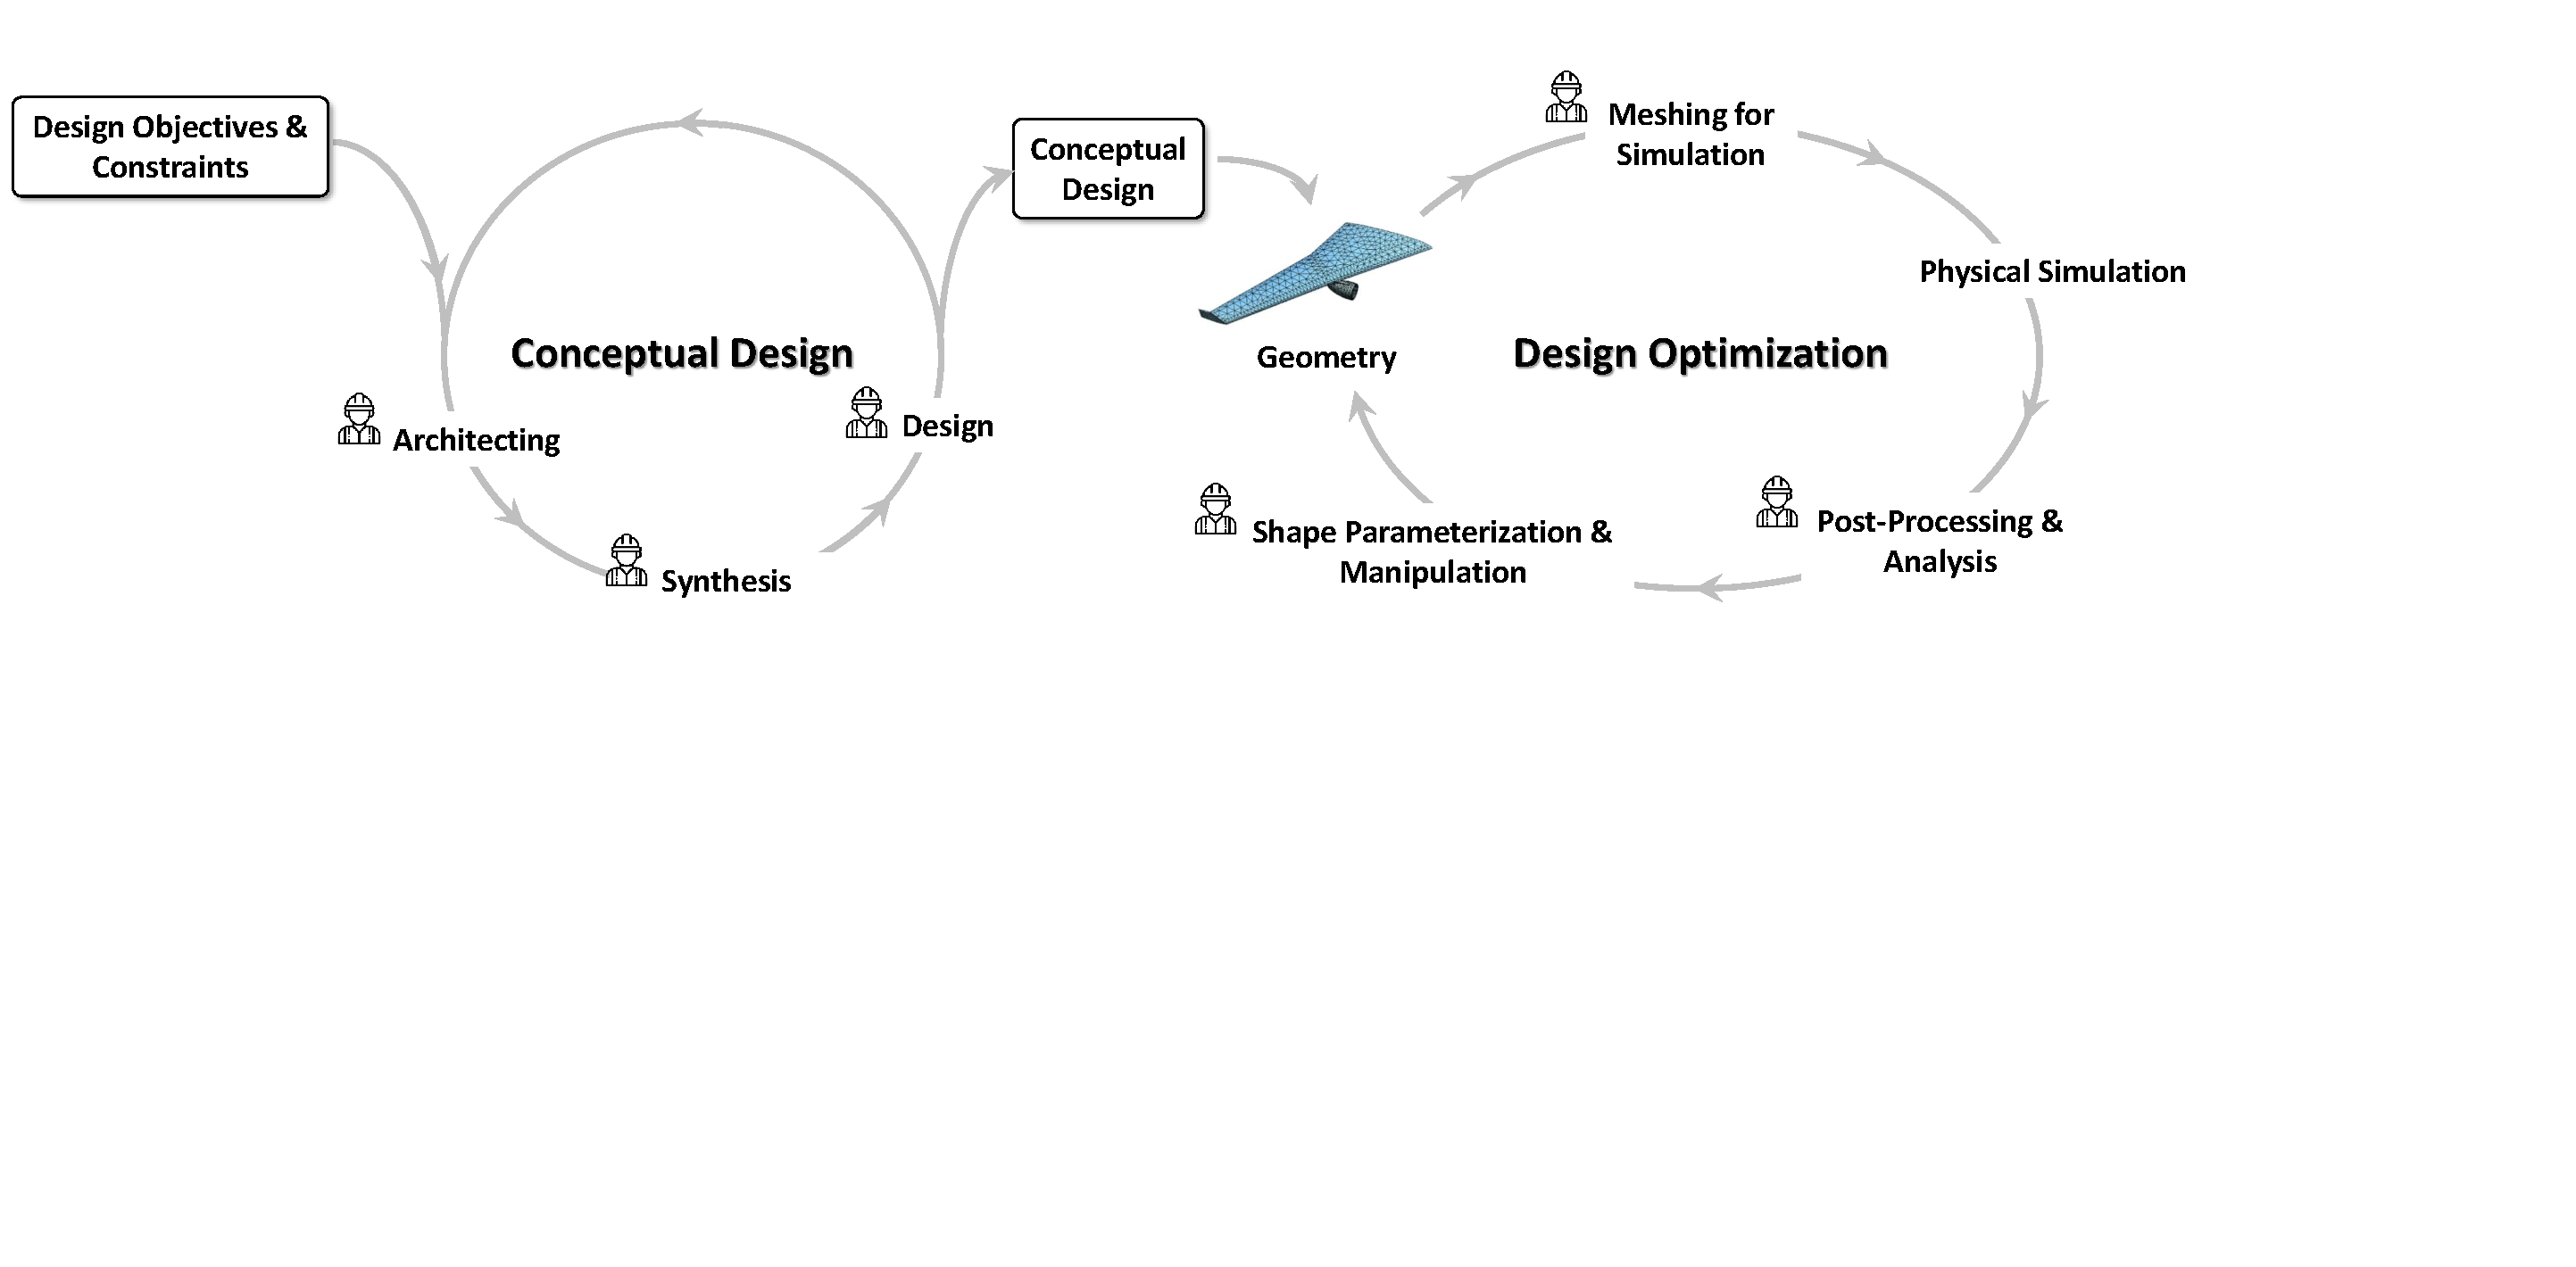
\includegraphics[width=1\linewidth]{chapter1/fig/traditional_framework.pdf}
    \end{center}
    \vspace{-3mm}
    \caption{
        \small The traditional, labor-intensive engineering design pipeline, characterized by serial workflows with many manual steps, inefficiency and high costs.
    }
    \label{ch1:fig:traditional_framework}
\end{figure}

% Opportunity of AI
Recent advances in artificial intelligence (AI) and machine learning offer promising opportunities to address these challenges in CAD/CAE. By leveraging data-driven models, AI can capture complex relationships in high-dimensional engineering data that traditional physics-based models might miss. By leveraging data-driven models, AI can capture complex relationships in high-dimensional engineering data that traditional physics-based models might miss. For example, AI methods can learn directly from simulation data to predict performance metrics, or learn from past designs to suggest new shape modifications--thereby accelerating the analysis and optimization of complex systems. Integrating AI into CAE has become a clear trend: AI can augment or even replace parts of the classical design workflow to improve efficiency. For instance, surrogate models can map design variables to predicted performance metrics (e.g. forces, efficiencies, noise) at low latency, supporting rapid evaluations in digital twin systems and enabling both gradient-based and gradient-free optimizations to `open up' black-box design objectives. Data-driven shape parameterization models such as Auto-Encoders and Variational Auto-Encoders (VAEs) learn compact design representations for efficient exploration with reduced dimensionality. Modern generative AI techniques like GANs can sample diverse, valid shapes under specified conditions, seeding design exploration and focusing search toward feasible regions. In summary, AI-driven approaches promise to search wider and faster in the design space than traditional methods, offering significant advantages in early-stage design exploration and optimization.

% scope of this thesis, and challenges
\section{Challenges in Engineering Design}
Within the broad field of AI-for-Design, this thesis zeroes in on a systematic study of a novel AI-driven design framework grounded in deep geometric learning for Aerodynamic Shape Design and Optimization (ASDO). Aerodynamic shapes (such as aircraft wings, airfoils, or turbomachinery blades) pose a unique challenge: they require a high-fidelity geometric representation that is compatible with physics-based analyses (e.g. enabling CFD mesh generation) and is also amenable to design optimization. Unfortunately, the traditional design workflow for such shapes has become unaffordable for small businesses and other resource-limited groups due to its complexity and cost. Meanwhile, prior applications of AI in this domain have been fragmented and often limited to monolithic, black-box solutions. These tend to demand extremely large training datasets and can be unreliable on out-of-distribution designs, leading to limited generalization and robustness. Their black-box nature also constrains modularity, interpretability and seamless integration with legacy workflows~\cite{aa.Lupp2025}.

Within this scope, ASDO faces five persistent obstacles that motivate the directions of this research. These obstacles can be grouped into (i) structural challenges of the traditional CAD/CAE workflow (T1, T2) and (ii) remaining gaps in prior AI-based approaches (T3-T5):
\begin{itemize}
    \item[T1.] \textbf{Heavy labor participation:} Extensive manual intervention and specialized domain knowledge are required at multiple stages, including the integration of multidisciplinary knowledge during conceptual design, ad-hoc shape parameterization to balance design freedom and optimization feasibility, and tedious processing to ensure consistency between geometries and their computational meshes for simulation.
    \item[T2.] \textbf{Constraints to low dimensionality:} Human-driven design is often confined to a limited number of design variables and objectives. This forces designers to simplify and divide the design problem, and ultimately accept a compromise in the breadth and depth of design space exploration.
    \item[T3.] \textbf{Data hunger:} Prior AI models typically require extensive, representative datasets of both geometries and simulations for training. In engineering practice, such large datasets are often infeasible to obtain due to cost, data sparsity or confidentiality.
    \item[T4.] \textbf{Limited generalization and robustness:} Data-driven models inherently introduce approximation errors and can become unreliable when facing scenarios outside the training distribution. This raises concerns in the reliability of design tasks.
    \item[T5.] \textbf{Monolithic generative models with poor controllability:} End-to-end black-box generative AI models amplify the above weaknesses. Their data hunger and weak generalization abilities, combined with limited conditioning inputs, result in poor controllability--they typically only accept a few low-dimensional control values, making it hard to enforce fine-grained design constraints.
\end{itemize}

% thesis ideas
\section{Thesis Scopes}
\label{ch1:sec:scopes}
\begin{figure}[tbh]
    \begin{center}
        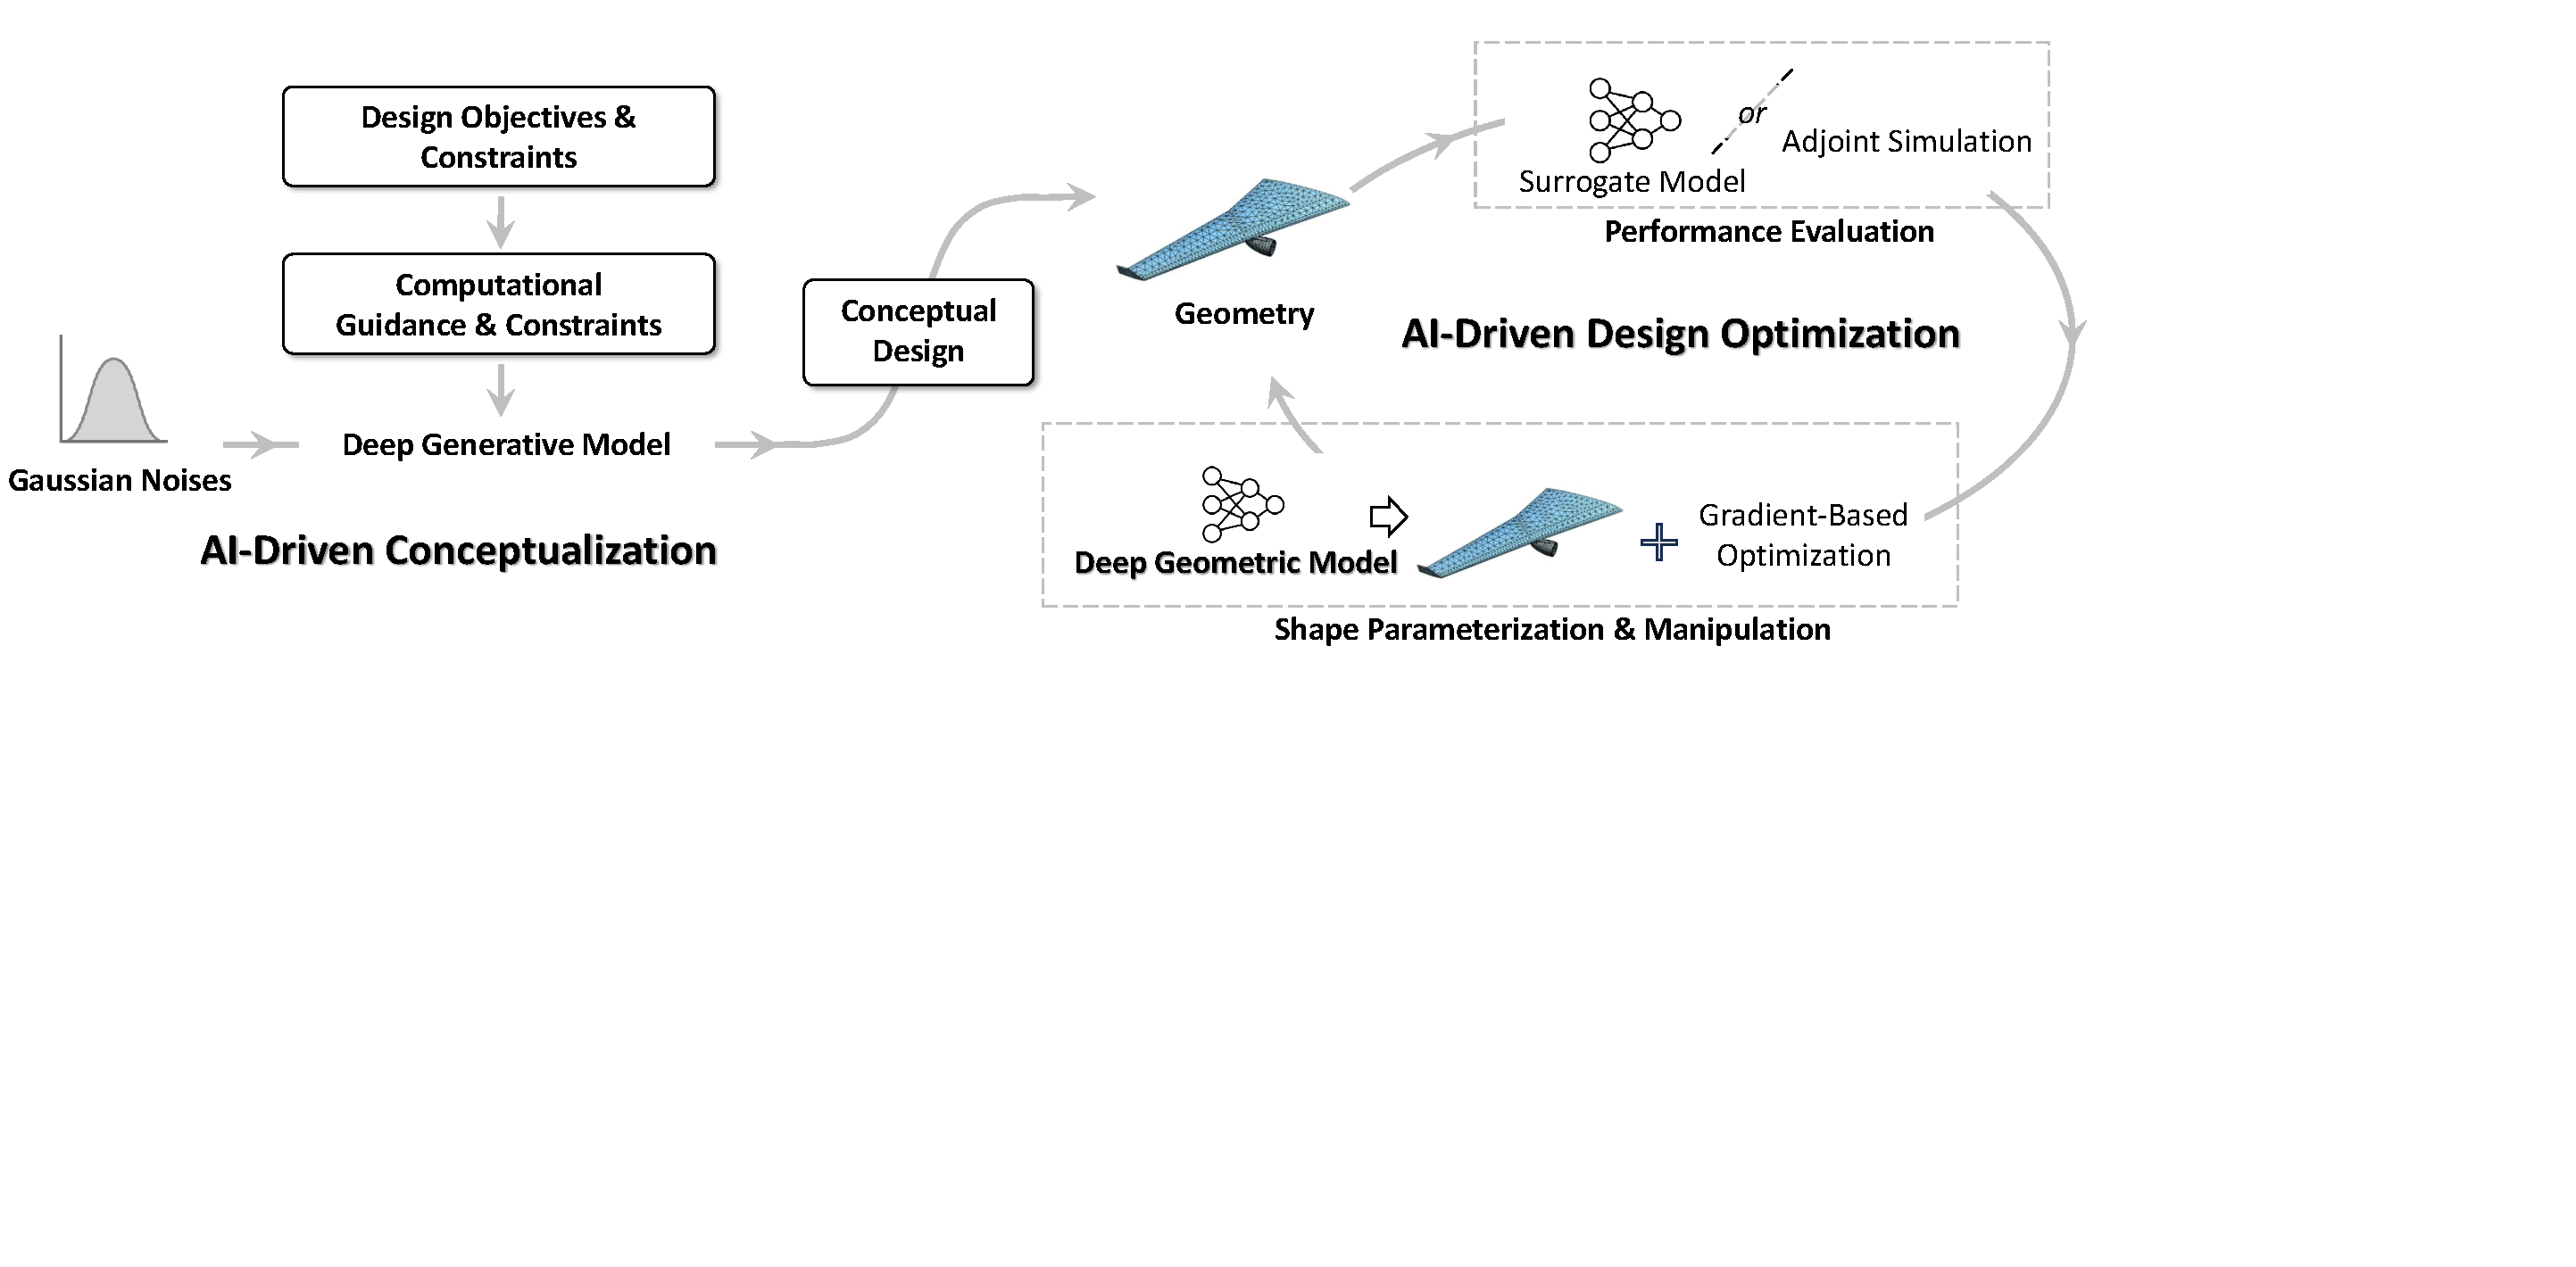
\includegraphics[width=1\linewidth]{chapter1/fig/ai_framework.pdf}
    \end{center}
    \vspace{-3mm}
    \caption{
        \small The proposed AI-driven engineering design pipeline, integrating deep geometric learning models developed in this thesis.
    }
    \label{ch1:fig:ai_framework}
\end{figure}

To address these challenges, this thesis proposes a systematic solution comprising two key stages (illustrated in Figure~\ref{ch1:fig:ai_framework}): 
\begin{itemize}
    \item[1.] \textbf{AI-driven conceptual design via controllable generative sampling:} Use a generative model to rapidly explore valid and diverse shape concepts under complex geometric and physics constraints.
    \item[2.] \textbf{High-fidelity design optimization with deep geometric parameterizations:} Starting from the generative solutions, perform automated aerodynamic shape optimization at high fidelity by using differentiable shape parameterizations that tightly couple the geometry and the computational mesh.
\end{itemize}

In the first stage, the generative model is intended to explore the design space broadly while respecting constraints. Notably, the generative model requires only a minimal amount of training data, orders of magnitude less than what prior AI models typically demand. Constraints (e.g., geometric or physical feasibility criteria) can be imposed on an initially unconditional generator in a plug-and-play, training-free manner.
In the second stage, the candidate designs produced by the generative model serve as starting points for further design optimization. This downstream optimization is highly automated: no additional training data, hyperparameter tuning or manual mesh processing is required during this phase. The same AI models can be applied across various ASDO tasks without human intervention, yet still achieve performance comparable to the best hand-tuned approaches in a traditional workflow. 
In summary, the emphasis on data-efficiency and automation yields an AI-driven design workflow that augments established practice while remaining practically deployable.

% research questions
This thesis investigates the above workflow through several research questions, each mapped to a core thesis chapter:
\begin{itemize}
    \item[Q1.] \textbf{Representation: } How to learn a low-dimensional, differentiable shape representation directly computational meshes, so that gradients directly flow to geometry?
    \item[Q2.] \textbf{Parameterization Choice: } When does a latent-space model versus a direct mapping model offer better exploration/control of shape designs, and how to generically regularize volumetric mesh deformations for either approach?
    \item[Q3.] \textbf{Automating Design Optimization at Scale: } Can a data-independent AI model eliminate the need for manual parameter tuning and computational mesh deformation, while still achieving high-fidelity ASDO performance?
    \item[Q4.] \textbf{Generative Exploration:} How to sample valid, diverse aerodynamic shapes from a small dataset of designs while adhering to fine-grained geometric requirements?
    \item[Q5.] \textbf{Physics-Guided Generation:} How to inject physical design objectives into the generative sampling process to achieve high-performance designs with less computational cost, and without retraining the generator for each new objective?
\end{itemize}

% thesis contributions
\section{Overview of Contributions}
This thesis addresses the above research questions through five core contributions, each corresponding to a chapter. In sequence, these contributions progressively build a complete pipeline from differentiable shape representation to performance-driven generative design.

\begin{itemize}
    \item \textbf{Chapter~\ref{ch3}--Learning Latent Representations of CFD Meshes.} The first contribution develops an auto-decoder neural network that learns a latent shape representation for computational fluid dynamics (CFD) meshes of airfoils. By training on a dataset of 2D airfoil geometries (each paired with its CFD mesh), the model compresses each mesh into a low-dimensional code and learns to reconstruct the mesh from that code by deforming a fixed template mesh. this work incorporates a novel volumetric mesh deformation regularization, which is devised to ensure the entire CFD mesh, including both the surface and volumetric computational cells, deforms smoothly and remains valid. This latent code thus parameterizes the airfoil’s shape while remaining fully differentiable. As a result, the CFD mesh becomes differentiable with respect to the shape parameters, enabling efficient gradient-based optimization through the mesh itself by allowing gradients to propagate from simulation outputs back to geometry.

    \item \textbf{Chapter~\ref{ch4}--Comparing Latent Space and Direct Mapping Models for Parameterization.} The second contribution explores two alternative strategies for automatic shape parameterization using deep geometric learning, and provides a comparative analysis. This work introduces: (i) a Latent Space Model (LSM), which generalizes the approach of Chapter~\ref{ch3}; and (ii) a Direct Mapping Model (DMM), a new approach that constructs a parameterization on the fly using only a single geometry, i.e. the design of interest. The DMM does not require any prior shape database. Both LSM and DMM incorporate the volumetric mesh deformation regularization, extending the technique from Chapter~\ref{ch3} in a mesh-free, more flexible fashion. These parameterizations are validated on 2D airfoil design problems by performing shape optimizations to compare their efficacy. Chapter~\ref{ch4} discusses the trade-offs between LSM and DMM: LSM leverages prior knowledge from the training dataset, whereas DMM is data-independent and is useful when a database is not available. This chapter provides guidance on choosing a parameterization approach, and sets the stage for designing a unified solution that combines the strengths of both methods.

    \item \textbf{Chapter~\ref{ch5}--DeepGeo: Deep Geometric Mapping for Shape Parameterization.} Building on insights from the first two contributions, the third contribution introduces DeepGeo, an automated shape parameterization framework geared towards high-fidelity aerodynamic shape optimization. DeepGeo can be seen as an evolution of the DMM concept, extended to handle complex 3D geometries and very large design spaces. Unlike traditional parameterization methods that require carefully tuning hyperparameters and constraining deformations, DeepGeo learns the deformation basis automatically, providing large deformation freedom while inherently maintaining global shape smoothness. This effectively streamlines the ASDO pipeline. In Chapter~\ref{ch5}, DeepGeo is validated in several case studies: a 2D circle optimization problem, the NASA Common Research Model (CRM) wing benchmark, and a blended-wing–body aircraft concept. Across these cases, DeepGeo achieves effective optimization results, matching or improving upon the best results obtained with state-of-the-art manual parameterization. These studies demonstrate DeepGeo’s potential to automate aerodynamic shape optimization, significantly reducing the manual effort traditionally involved in setup while still delivering high-performance designs.

    \item \textbf{Chapter~\ref{ch6}--DiffGeo: Latent-Space Diffusion for Generative Design Space Exploration.} After establishing methods for parameterizing and optimizing a single design, this thesis shifts focus to generative design space exploration. The fourth contribution, DiffGeo, introduces a deep generative model that learns to sample aerodynamic shapes. The core idea is to train a denoising diffusion model on the latent representations learned by the auto-decoder from Chapter~\ref{ch3}. This approach proves highly data-efficient, requiring far fewer training shapes than GAN-based generators reported in the literature. Additionally, the latent parameterization used by DiffGeo ensures that every sampled shape is valid, an important advantage over naive generative methods. Chapter~\ref{ch6} also demonstrates a form of conditional generation that guides the diffusion model to produce shapes with specified geometric properties, without needing to retrain the generator for each new condition, highlighting the flexibility of this approach. The DiffGeo framework thus lays groundwork for AI-driven concept generation in ASDO, providing engineers with a toolkit to sample novel designs that meet certain criteria, which can then be screened or fine-tuned. This contribution illustrates how deep generative learning can tackle the exploration aspect of design, complementing the optimization focus of earlier chapters.

    \item \textbf{Chapter~\ref{ch7}--Physics-Guided Generative Design Space Exploration.} The final technical contribution combines generative modeling and physics-based design objectives by introducing Dfow-SUR, a method for physics-guided generative design. In this approach, a surrogate model is used as a guide or reward signal during shape generation. Specifically, we fully differentiate through the diffusion generation process to optimize the latent sampling with respect to the surrogate’s output. Compared to previous conditioning mechanisms for diffusion models, Dfow-SUR achieves significantly better controllability and computational efficiency. Chapter~\ref{ch7} demonstrates that Dfow-SUR can produce airfoil and wing designs with improved aerodynamic metrics. This approach highlights a possible future for AI-driven design workflows: the generative model proposes candidate designs, and a physics-informed optimization refines them, so that we can move closer to an autonomous design system that relies on minimal human input.
\end{itemize}

% connections
\begin{figure}
    \centering
    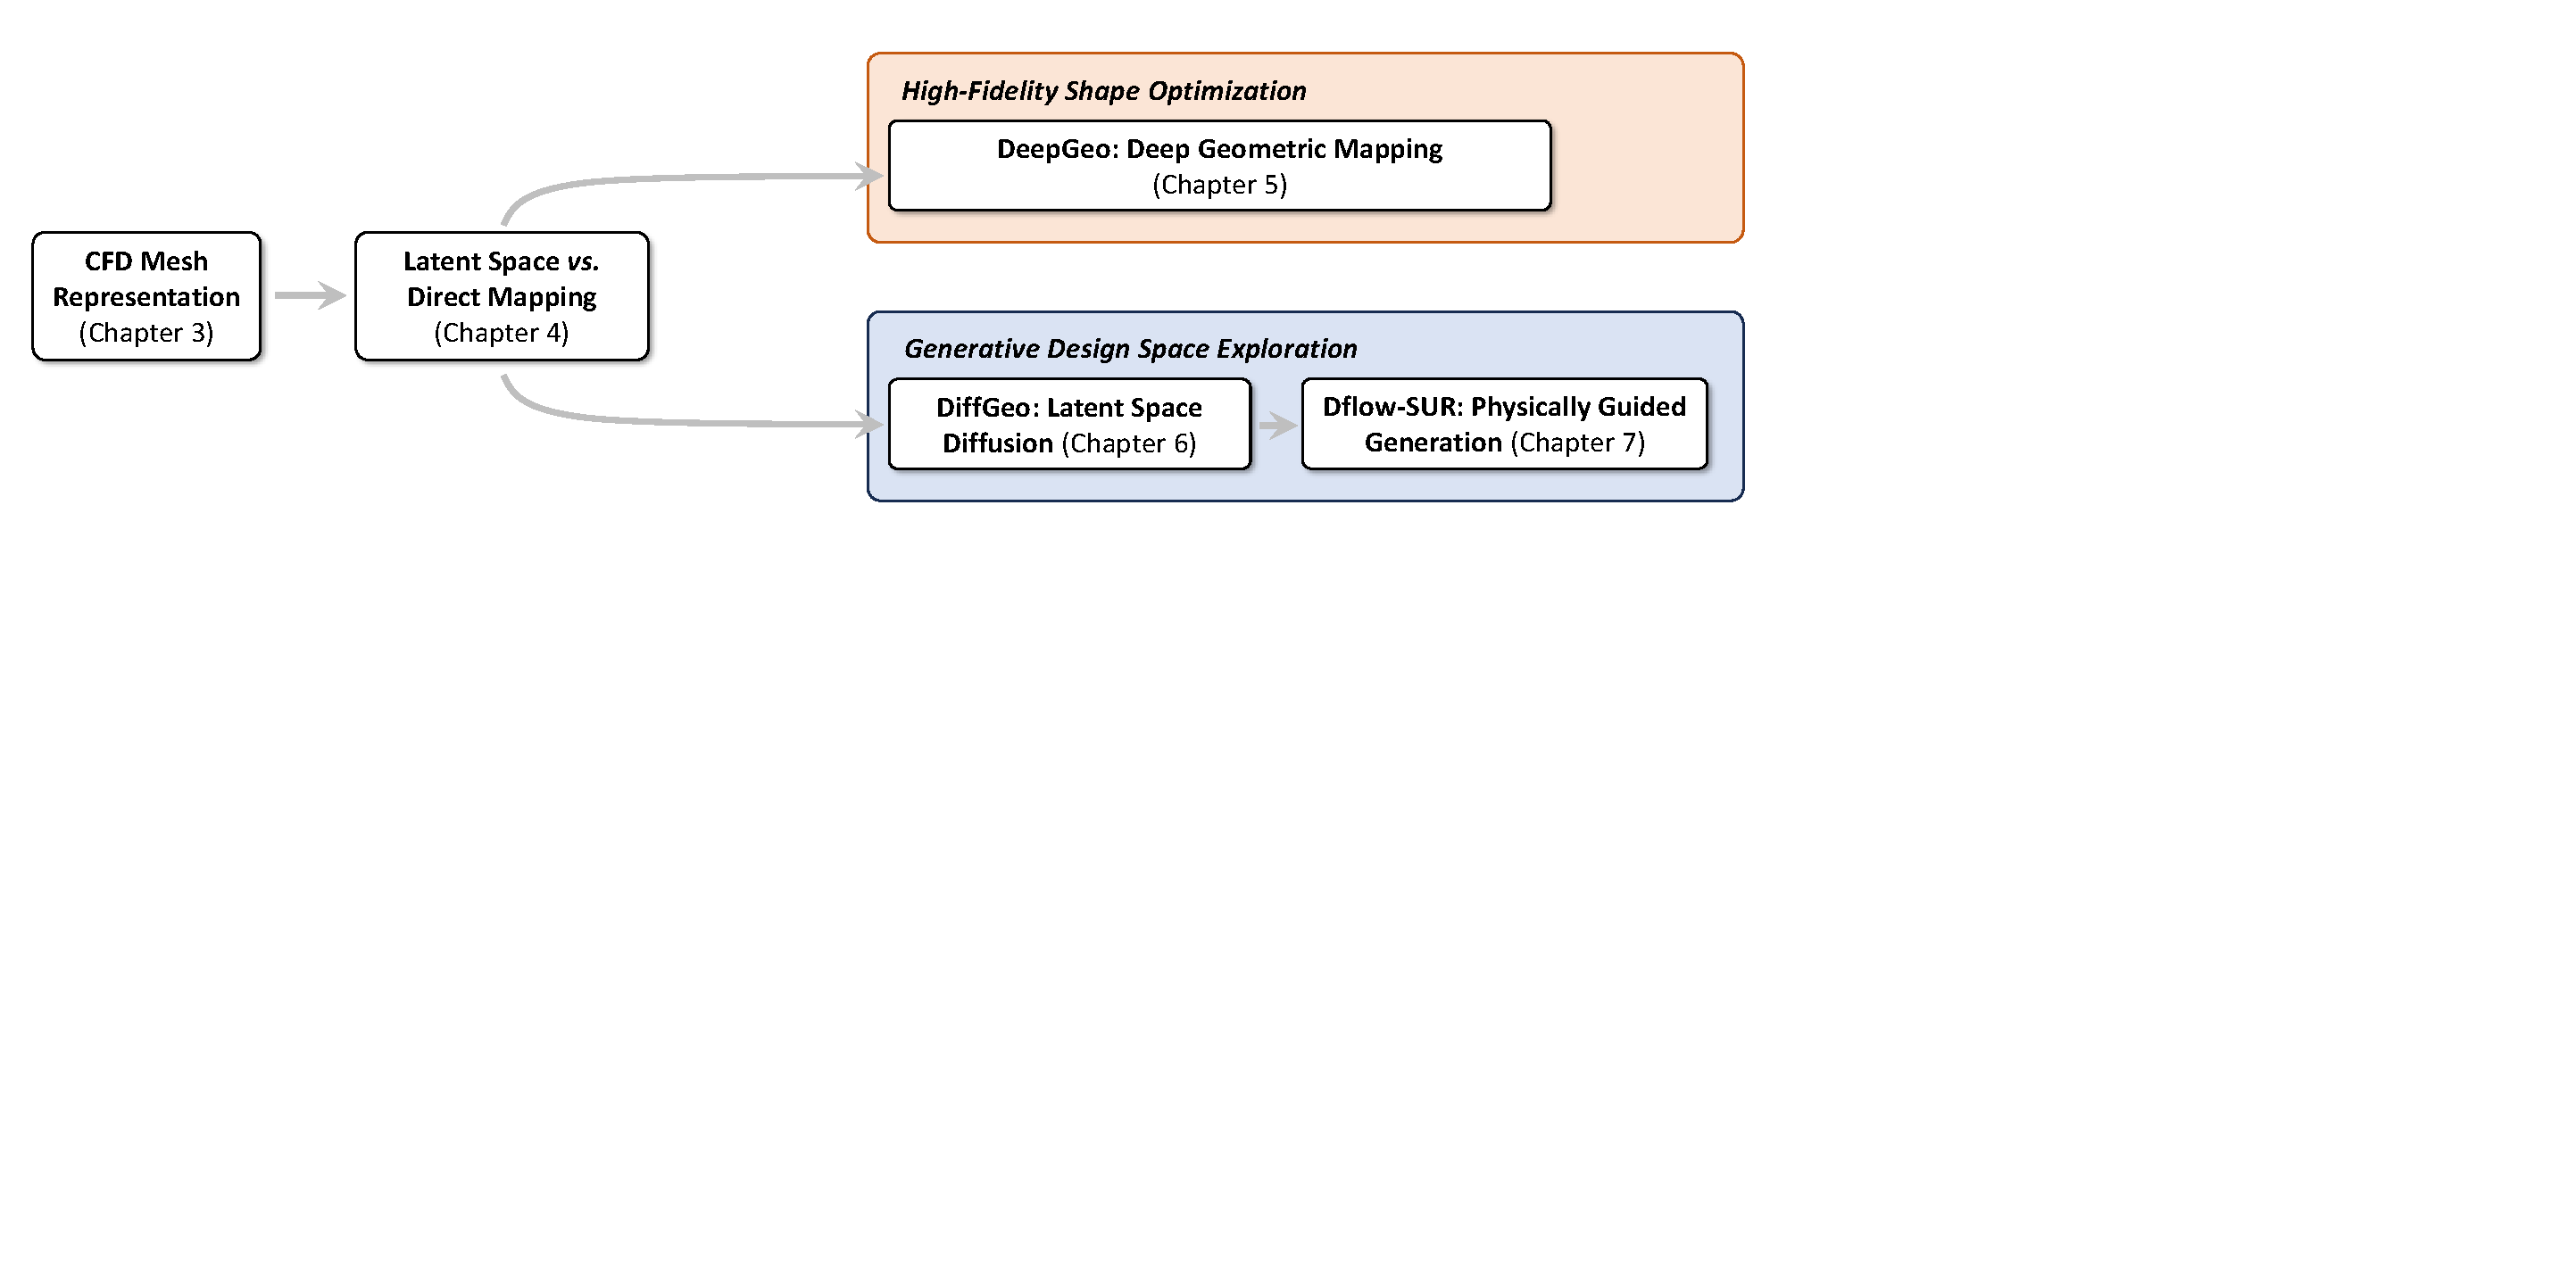
\includegraphics[width=0.98\linewidth]{chapter1/fig/evolution.pdf}
    \caption{The progression of chapters in this thesis.}
    \label{ch1:fig:evolution}
\end{figure}

The progression of chapters above reflects the evolving focus of this research. As illustrated in Figure~\ref{ch1:fig:evolution}, it began by addressing the fundamental bottleneck of design optimization: the lack of a good parameterization, by learning latent representations (Chapter~\ref{ch3}). Then this geometric model with the same mesh regularization technique diverges: a more flexible direct mapping approach was introduced (Chapter~\ref{ch4}), which was subsequently scaled up to complex, real-world configurations via DeepGeo (Chapter~\ref{ch5}). Then the focus of latent space model shifts towards design space exploration: first by efficiently sampling the latent space with comprehensive benchmarking with prior generative models (Chapter~\ref{ch6}), and finally by guiding generation with performance evaluations (Chapter~\ref{ch7}). Each stage built on the insights of the previous ones. In this way, the thesis work transitioned from developing design enablers (DeepGeo) to developing design creators (DiffGeo, Dfow-SUR), all under the unifying theme of deep geometric learning for engineering design. 

\begin{figure}[!tbh]
    \begin{center}
        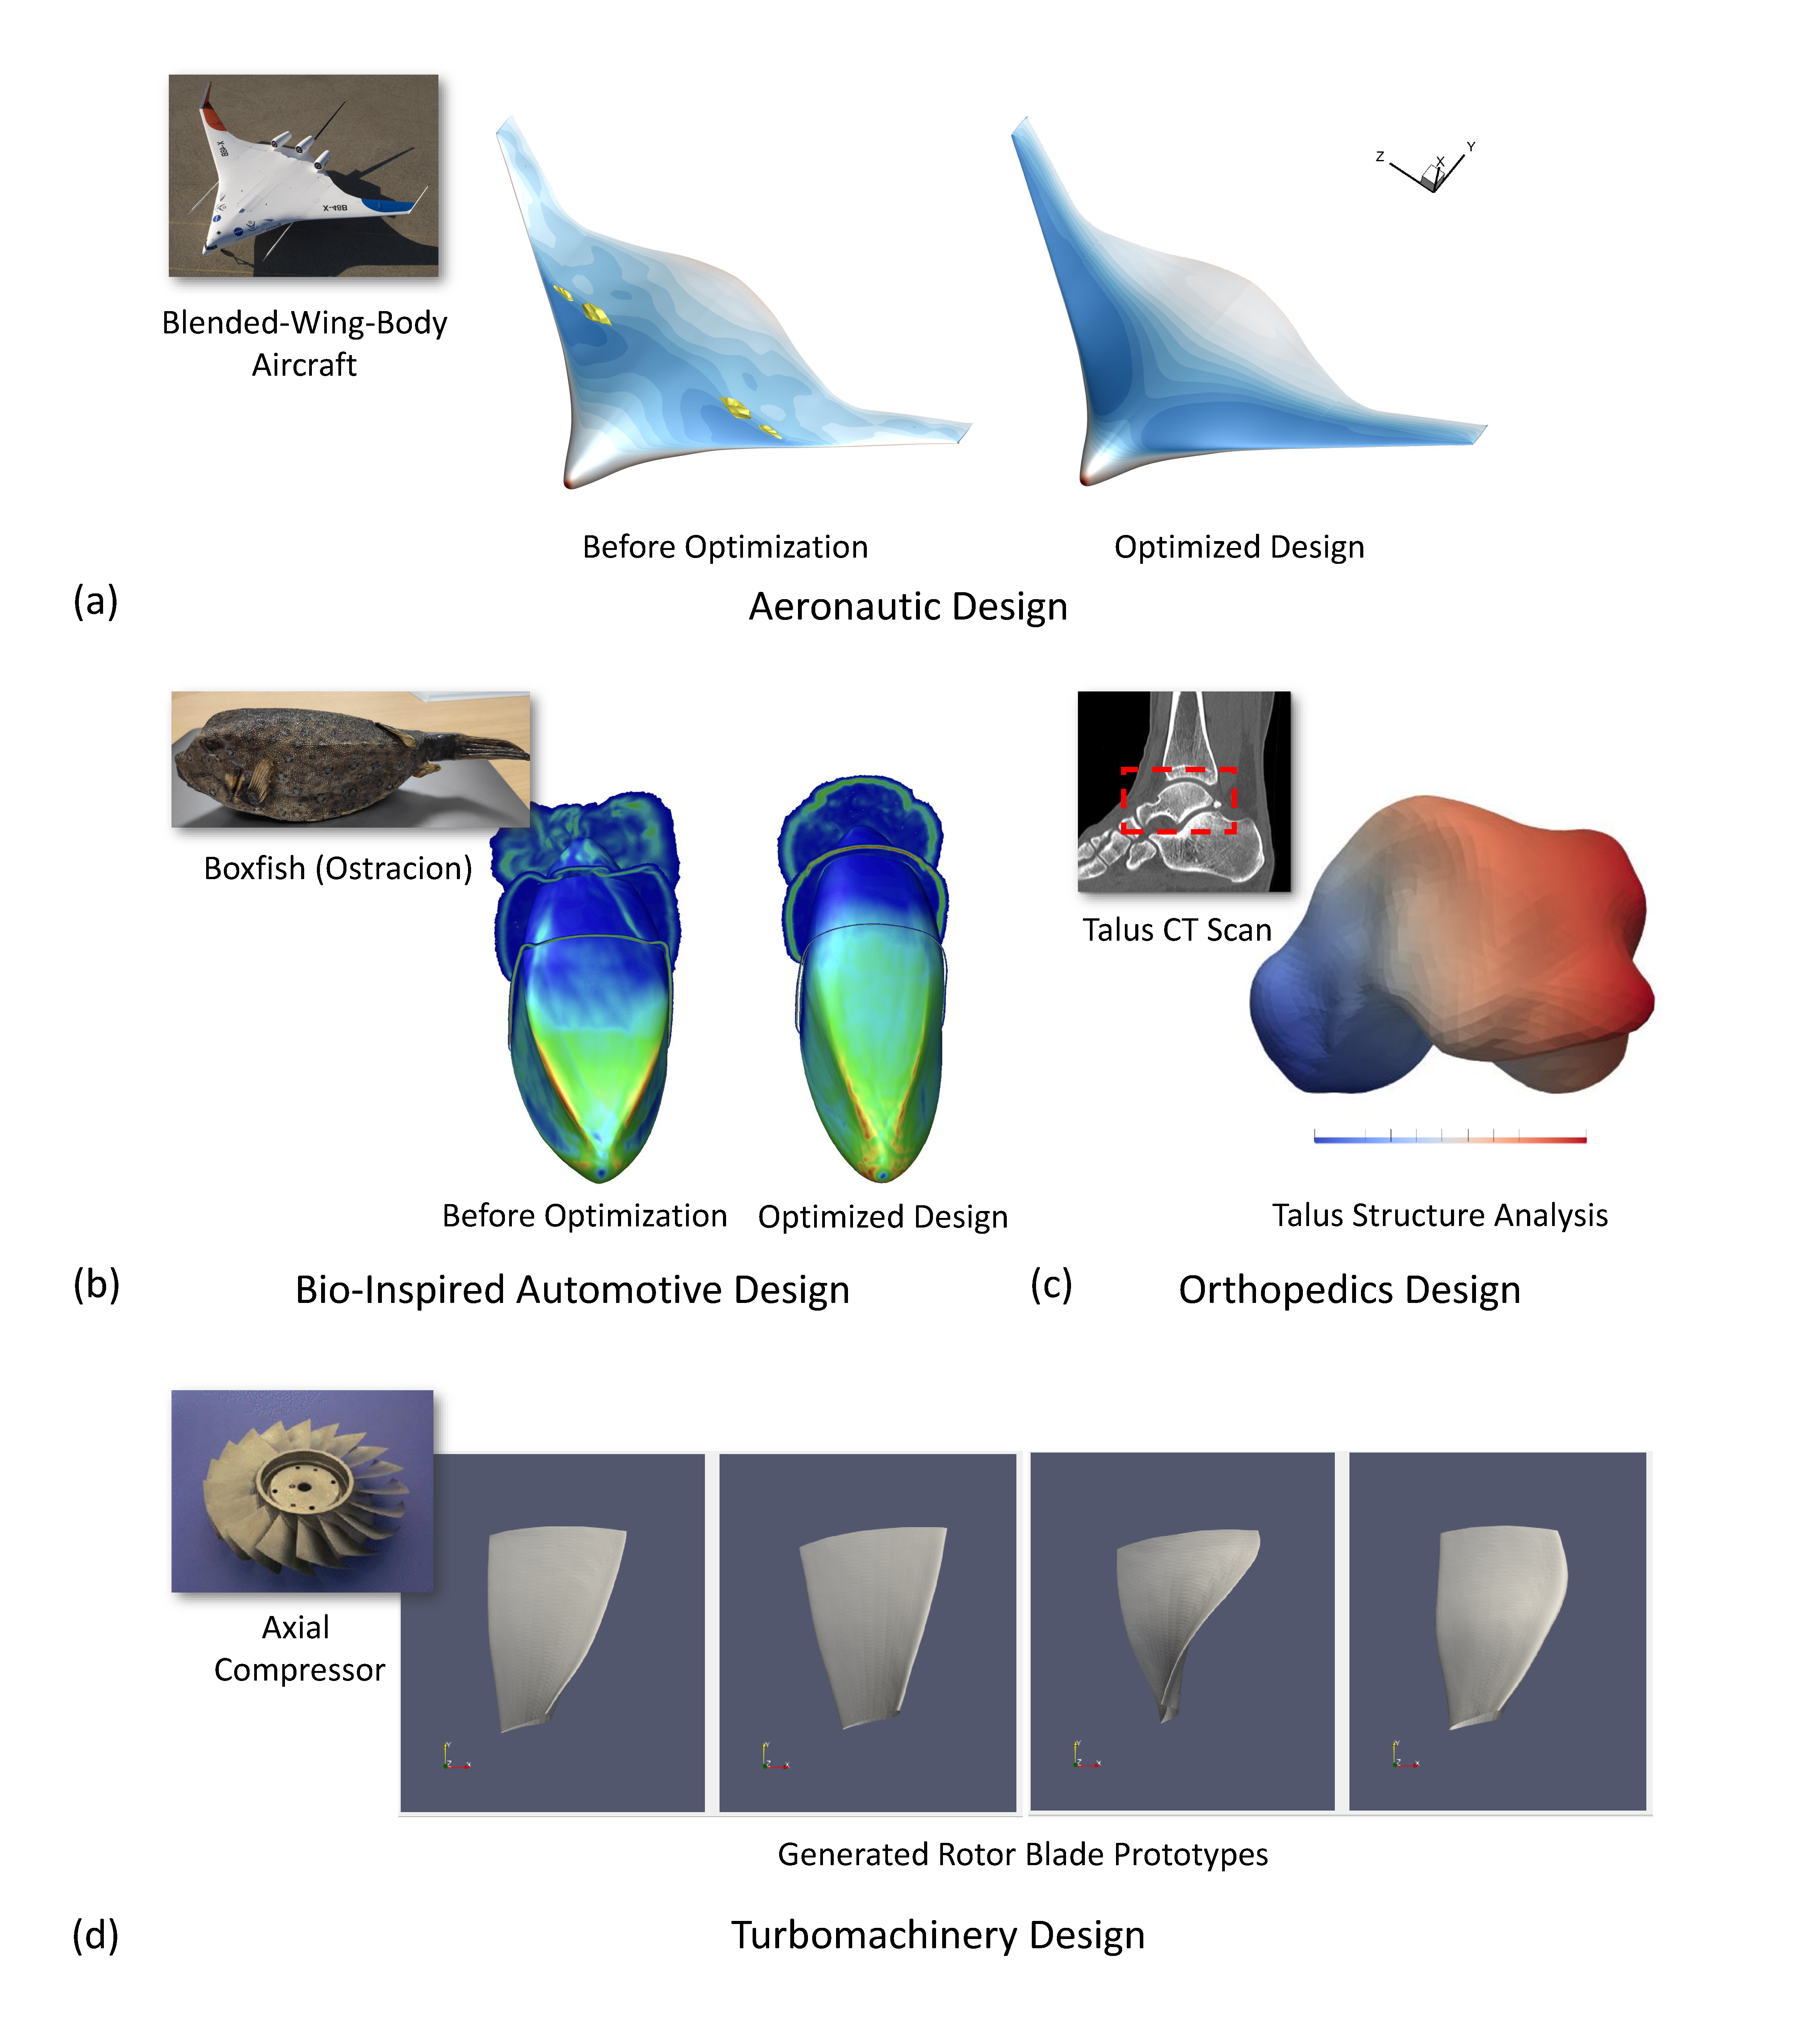
\includegraphics[width=1\linewidth]{chapter1/fig/teaser.pdf}
    \end{center}
    \vspace{-3mm}
    \caption{
        \small Diverse applications enabled by the deep geometric learning models developed during my PhD study. These include design cases in (a) aeronautics (aircraft optimization), (b) automotive (bio-inspired car body design), (c) orthopedics (patient-specific talus modeling) and (d) turbomachinery (rotor blade prototyping).
    }
    \label{ch1:fig:teaser}
\end{figure}

\section{Implications and Broader Impact}
The methods presented in this thesis bring multiple broader implications for engineering design:
\begin{itemize}
    \item \textbf{Accelerated concept exploration and design cycle:} The diffusion-based generative AI models developed can produce diverse, valid design candidates for expert evaluation and inspiration during the early conceptual stage. Rather than replacing downstream optimization, this rapid concept generation complements it by providing better starting points. Meanwhile, the design optimization itself is simplified and accelerated by the highly automated parameterization models, reducing the need for ad-hoc and repetitive human intervention. The overall design cycle can be significantly shortened. Design iteration and innovation are expected to accelerate in industrial practice.

    \item \textbf{Path toward multi-physics workflows:} Although the work in this thesis focuses mainly on single-physics (aerodynamic) phenomena, the underlying framework is extendable to multi-physics problems. The developments here pave the way toward fully AI-driven Multidisciplinary Design Optimization (MDO), where multiple physics (e.g. aerodynamic, structural, material) are integrated into a unified generation-and-optimization pipeline.

    \item \textbf{Practical and data-efficient AI:} By emphasizing data-efficiency, the cutting-edge AI techniques developed become far more practical in real-world engineering scenarios, where data is often scarce, noisy or proprietary. This improved efficiency can help democratize advanced CAD/CAE capabilities, making design optimization accessible to small businesses and other groups with limited resources.
\end{itemize}

In summary, the approaches in this thesis aim to augment human designers with AI tools that handle the heavy lifting of geometry manipulation and concept generation. This human-AI collaboration can lead to faster design iterations, reduced development costs and more innovative results. While challenges remain, the trajectory outlined by this work points to a design process that is more exploratory, efficient and tightly integrated with computational physics. This has implications not only for aeronautical design but for any engineering domain where complex geometries and simulations intersect (e.g., automotive, orthopedics, turbomachinery, as shown in Figure~\ref{ch1:fig:teaser}). By accelerating and automating key parts of the design loop, engineers can devote more time to creative thinking and rigorous validation, ultimately pushing the boundaries of engineering design.

\section{Publications and Works in Progress}
This thesis has led to the following publications (including those under review at the time of writing):

\textbf{Zhen Wei}, Benoît Guillard, Pascal Fua, Vincent Chapin, and Michaël Bauerheim, “Latent Representation of Computational Fluid Dynamics Meshes and Application to Airfoil Aerodynamics,” AIAA Journal, 2023. https://doi.org/10.2514/1.J062533.

\textbf{Zhen Wei}, Pascal Fua, and Michaël Bauerheim, “Automatic Parameterization for Aerodynamic Shape Optimization via Deep Geometric Learning,” in AIAA Aviation Forum, 2023. https://doi.org/10.2514/6.2023-3471.

\textbf{Zhen Wei}, Aobo Yang, Jichao Li, Michaël Bauerheim, Rhea P. Liem, and Pascal Fua, "DeepGeo: Deep Geometric Mapping for Automated and Effective Parameterization in Aerodynamic Shape Optimization,” in AIAA Aviation Forum, 2024. https://doi.org/10.2514/6.2024-3839. [Best Student Paper in MDO, 2024 AIAA Aviation Forum][2024 AIAA MDO Best Paper]

\textbf{Zhen Wei}, Edouard R. Dufour, Colin Pelletier, Pascal Fua, and Michaël Bauerheim, “Diffairfoil: An efficient novel airfoil sampler based on latent space diffusion model for aerodynamic shape optimization,” in AIAA AVIATION Forum, 2024, https://doi.org/10.2514/6.2024-3755.

\textbf{Zhen Wei}, Aobo Yang, Jichao Li, Michaël Bauerheim, Rhea P. Liem, and Pascal Fua, “Automated Parameterization for Aerodynamic Shape Optimization via Deep Geometric Learning,” AIAA Journal, 2025. https://doi.org/10.2514/1.J065203.

\textbf{Zhen Wei}, Edouard R. Dufour, Colin Pelletier, Pascal Fua, and Michaël Bauerheim, "Aerodynamic Shape Design Space Exploration with Deep Latent Diffusion Model," in submission.

Aobo Yang, \textbf{Zhen Wei}, Rhea P. Liem, Pascal Fua, “Dflow-SUR: Enhancing Generative Aerodynamic Inverse Design using Differentiation Throughout Flow Matching,” in submission.

